% ============================================================
%  Plataforma de Badges da Softinsa — Relatório
%  Template com as cores do projeto
% ============================================================
\documentclass[12pt,a4paper]{report}

% --- Encoding & Language ---
\usepackage[utf8]{inputenc}
\usepackage[T1]{fontenc}
\usepackage[portuguese]{babel}

% --- Geometry ---
\usepackage[
  top=2.5cm,
  bottom=2.5cm,
  left=3cm,
  right=2.5cm
]{geometry}

% --- Fonts ---
\usepackage{mathptmx}
\usepackage{microtype}
\usepackage{indentfirst}

% --- Line Spacing ---
\usepackage{setspace}
\onehalfspacing

% --- Colors (from project palette) ---
\usepackage{xcolor}
\definecolor{primary}{HTML}{00B8E0}        % --color-primary
\definecolor{secondary}{HTML}{39639C}      % --color-secondary
\definecolor{onprimary}{HTML}{FFFFFF}      % --color-on-primary
\definecolor{primarycontainer}{HTML}{B9EBF6}% --color-primary-container
\definecolor{background}{HTML}{FDF7FF}     % --color-background
\definecolor{onsurface}{HTML}{171C1E}      % --color-on-surface
\definecolor{outline}{HTML}{70787C}        % --color-outline

% --- Graphics & Floats ---
\usepackage{graphicx}
\usepackage{float}
\usepackage{caption}
\captionsetup{
  font=small,
  labelfont={bf,color=secondary},
  textfont={color=onsurface},
  position=below
}
\captionsetup[table]{position=below}
\captionsetup[figure]{position=below}

% --- Tables ---
\usepackage{booktabs}
\usepackage{tabularx}

% --- Lists ---
\usepackage{enumitem}

% --- Hyperlinks ---
\usepackage{hyperref}
\hypersetup{
  colorlinks=true,
  linkcolor=secondary,
  citecolor=secondary,
  urlcolor=primary,
  bookmarksnumbered=true
}

% --- Headers & Footers ---
\usepackage{fancyhdr}
\pagestyle{fancy}
\fancyhf{}
\fancyhead[L]{\small\color{outline}\leftmark}
\fancyhead[R]{\small\color{outline}\thepage}
\renewcommand{\headrulewidth}{0.4pt}
\renewcommand{\headrule}{\hbox to\headwidth{\color{primary}\leaders\hrule height \headrulewidth\hfill}}
\fancyfoot[C]{\small\color{outline}Plataforma de Badges da Softinsa}

% --- Chapter & Section Styling ---
\usepackage{titlesec}

\titleformat{\chapter}[display]
  {\normalfont\Huge\bfseries\color{secondary}}
  {\colorbox{primary}{\parbox{1.5cm}{\centering\color{onprimary}\fontsize{48}{52}\selectfont\thechapter}}}
  {20pt}
  {}

\titleformat{\section}
  {\normalfont\Large\bfseries\color{secondary}}
  {\thesection}{1em}{}
  [\vspace{2pt}{\color{primary}\hrule height 1.5pt}]

\titleformat{\subsection}
  {\normalfont\large\bfseries\color{secondary!80!black}}
  {\thesubsection}{1em}{}

% --- Code Listings ---
\usepackage{listings}
\lstset{
  basicstyle=\ttfamily\small,
  backgroundcolor=\color{primarycontainer!30},
  frame=single,
  rulecolor=\color{primary!50},
  keywordstyle=\color{secondary}\bfseries,
  commentstyle=\color{outline}\itshape,
  stringstyle=\color{primary!70!black},
  breaklines=true,
  tabsize=2
}

% --- Bibliography ---
\usepackage[style=numeric,sorting=nyt,backend=biber]{biblatex}
\addbibresource{referencias.bib}

% --- Glossary (optional) ---
% \usepackage[toc]{glossaries}
% \makeglossaries

% --- Custom Commands ---
\newcommand{\keyword}[1]{\textbf{\color{primary}#1}}
\newcommand{\role}[1]{\textit{\color{secondary}#1}}

% ============================================================
\begin{document}

% --- Cover Page ---
\begin{titlepage}
  \begin{center}

    \vspace*{0.5cm}

    % Logos
    
\includegraphics[height=2.5cm]{images/logo-escola.png}
    \hspace{2cm}
    
\includegraphics[height=2.5cm]{images/logo-softinsa.png}\\[1.5cm]

    {\color{primary}\rule{\textwidth}{2pt}}\\[0.6cm]

    {\fontsize{26}{32}\selectfont\bfseries\color{secondary}
      Plataforma de Badges da Softinsa}\\[0.5cm]

    {\fontsize{14}{18}\selectfont\color{onsurface}
      Relatório da Unidade Curricular de Projeto Integrado}\\[0.3cm]

    {\color{primary}\rule{\textwidth}{2pt}}\\[1.2cm]

    {\large\color{onsurface}
      Curso de Licenciatura em Engenharia Informática\\[0.3cm]
      Ano Letivo: 2.º}\\[1.8cm]

    {\Large\color{secondary}\bfseries
      Hugo Alexandre Pereira Afonso} {\large\color{outline}(pv30032)}\\[0.3cm]
    {\Large\color{secondary}\bfseries
      Mateus Valente Frias Silva} {\large\color{outline}(pv29989)}\\[0.3cm]
    {\Large\color{secondary}\bfseries
      Rodrigo de Almeida Martins} {\large\color{outline}(pv30773)}\\[0.3cm]
    {\Large\color{secondary}\bfseries
      Susana Daniela Tavares} {\large\color{outline}(pv27467)}\\[2cm]

    {\large\color{onsurface}
      Trabalho efetuado sob a orientação de:\\[0.3cm]
      \textbf{Artur Sousa}\\[0.15cm]
      \textbf{Júlio Florentino}}

    \vfill

    {\large\color{outline}
      Junho 2026}

  \end{center}
\end{titlepage}

% --- Numbering ---
\pagenumbering{roman}

% ============================================================
% Agradecimentos
% ============================================================
\chapter*{Agradecimentos}
\addcontentsline{toc}{chapter}{Agradecimentos}

Enquanto grupo, gostaríamos de manifestar o nosso sincero agradecimento aos professores Artur Sousa e Júlio Florentino pelo apoio, orientação e tempo que nos dedicaram ao longo deste trabalho.

Gostaríamos também de expressar a nossa gratidão à Softinsa, bem como a todos os que a representaram, principalmente o engenheiro Rui Costa, pelo tempo investido na elaboração do enunciado deste projeto.

\newpage

% ============================================================
% Resumo
% ============================================================
\chapter*{Resumo}
\addcontentsline{toc}{chapter}{Resumo}

% Escrever resumo aqui.

\vspace{1cm}
\noindent\textbf{Palavras-chave:} % gamificação, badges digitais, credenciais, ...

\newpage

% ============================================================
% Abstract (optional)
% ============================================================
\chapter*{Abstract}
\addcontentsline{toc}{chapter}{Abstract}

% Write abstract here.

\vspace{1cm}
\noindent\textbf{Keywords:} % gamification, digital badges, credentials, ...

\newpage

% ============================================================
% Lista de Abreviaturas
% ============================================================
\chapter*{Lista de Abreviaturas}
\addcontentsline{toc}{chapter}{Lista de Abreviaturas}

\begin{tabbing}
  \hspace{3cm}\= \kill
  \textbf{API}  \> Application Programming Interface \\[4pt]
  \textbf{AWS}  \> Amazon Web Services \\[4pt]
  \textbf{BD}   \> Base de Dados \\[4pt]
  \textbf{IBM}  \> International Business Machines \\[4pt]
  \textbf{JWT}  \> JSON Web Token \\[4pt]
  \textbf{KPI}  \> Key Performance Indicator \\[4pt]
  \textbf{LP}   \> Learning Path \\[4pt]
  \textbf{RGPD} \> Regulamento Geral sobre a Proteção de Dados \\[4pt]
  \textbf{SL}   \> Service Line \\[4pt]
  \textbf{SLA}  \> Service Level Agreement \\[4pt]
  \textbf{SLL}  \> Service Line Leader \\[4pt]
  \textbf{TM}   \> Talent Manager \\[4pt]
  \textbf{UC}   \> Unidade Curricular \\[4pt]
  \textbf{UI}   \> User Interface \\[4pt]
  \textbf{URL}  \> Uniform Resource Locator \\[4pt]
  \textbf{UX}   \> User Experience \\
\end{tabbing}

\newpage

% ============================================================
% Glossário
% ============================================================
\chapter*{Glossário}
\addcontentsline{toc}{chapter}{Glossário}

\begin{tabularx}{\textwidth}{@{}l@{\hspace{1em}}X@{}}
  \textbf{\color{secondary}Badge}                & Credencial digital verificável que atesta a obtenção de um determinado nível de competências ou a conclusão de requisitos específicos por parte do consultor. \\[6pt]
  \textbf{\color{secondary}Consultor}             & Perfil de utilizador da plataforma que representa o colaborador/técnico da Softinsa responsável por submeter evidências e progredir nos itinerários de aprendizagem. \\[6pt]
  \textbf{\color{secondary}Credly}                & Plataforma global de referência no mercado para a emissão, gestão e partilha de badges e certificações digitais. \\[6pt]
  \textbf{\color{secondary}Evidência}             & Documento digital (certificado, diploma, relatório em formato PDF, imagem ou outro) submetido pelo consultor que comprova a realização de um determinado requisito. \\[6pt]
  \textbf{\color{secondary}Gamificação}           & Aplicação de dinâmicas, mecânicas e elementos típicos de jogos (como sistema de pontos, conquistas especiais e rankings) num contexto corporativo para motivar a aprendizagem. \\[6pt]
  \textbf{\color{secondary}Learning Path}         & Estrutura macro de formação contínua dentro da empresa, que agrupa várias SLs e áreas técnicas. \\[6pt]
  \textbf{\color{secondary}Requisito}             & Meta ou curso específico associado a um determinado nível, cuja conclusão e validação são obrigatórias para obter o respetivo badge. \\[6pt]
  \textbf{\color{secondary}Service Line}          & Divisão interna da empresa que agrupa áreas de competências técnica afins. \\[6pt]
  \textbf{\color{secondary}Softinsa}              & Empresa do grupo IBM em Portugal, focada em serviços de consultoria tecnológica e gestão de aplicações, que forneceu o tema para este projeto integrado. \\[6pt]
  \textbf{\color{secondary}Workflow de Estados}   & Ciclo de vida sequencial pelo qual uma candidatura a um badge transita no sistema (compreendendo os estados `Open', `Submitted', `Em Validação' e `Fechado') consoante as ações dos avaliadores. \\
\end{tabularx}

\newpage

% ============================================================
% Table of Contents, Figures, Tables
% ============================================================
\tableofcontents
\newpage
\listoffigures
\newpage
\listoftables
\newpage

% --- Switch to arabic numbering ---
\pagenumbering{arabic}

% ============================================================
% Introdução
% ============================================================
\chapter{Introdução}
\label{ch:introducao}

O presente relatório documenta todo o processo de idealização, planeamento e implementação da Plataforma de Badges da Softinsa, a propósito da Unidade Curricular (UC) de Projeto Integrado. O tema do projeto foi concebido e fornecido pela Softinsa, com o propósito de desafiar os estudantes a desenvolverem uma solução tecnológica robusta e adaptada a uma necessidade real do contexto corporativo da empresa. Sendo o desenvolvimento deste ecossistema efetuado integralmente a partir do zero, este documento detalha as várias etapas do ciclo de vida do software, compreendendo a modelação conceptual do modelo de dados, a conceção da experiência e interface do utilizador (UI/UX) através de protótipos em Figma~\cite{figma}, e a subsequente codificação das três frentes da solução: a API REST~\cite{restapi} de backend, o portal Web e a aplicação Mobile (apenas para o perfil de consultor).

\section{Enquadramento e Motivação}

No atual panorama do setor das tecnologias da informação, a competitividade das empresas está intrinsecamente ligada à capacidade de valorização e atualização contínua do seu capital humano. Como empresa líder em consultoria tecnológica, a Softinsa reconhece que a formação contínua e a certificação de competências dos seus colaboradores são pilares fundamentais para sustentar o crescimento do negócio, responder às exigências do mercado e manter equipas de alto rendimento. Para organizar este esforço de capacitação, a empresa dispõe de múltiplos Learning Paths (LP), ou itinerários de aprendizagem, estruturados por Service Lines (SL) e áreas técnicas específicas, oferecendo uma progressão de carreira clara através de vários níveis de consolidação de conhecimento.

Contudo, a gestão manual e descentralizada destas formações -- frequentemente realizadas em plataformas externas como a Udemy, IBM, AWS ou Microsoft -- acarreta desafios operacionais significativos. Identificou-se uma clara dificuldade em evidenciar e validar de forma ágil as competências efetivamente adquiridas pelos consultores. Para responder a isto, o ecossistema da Softinsa exige um fluxo rigoroso de auditoria assente em papéis bem definidos: o Consultor, que executa as formações e submete as suas evidências; o Talent Manager (TM), responsável por uma primeira validação global e transversal dos documentos submetidos; e o Service Line Leader (SLL), que efetua a validação técnica e final com base na sua área específica de especialização. Todo este ecossistema é centralizado e parametrizado pelo perfil de Administrador, que faz a gestão de conteúdos e utilizadores da plataforma.

Atualmente, a ausência de um sistema automatizado e padronizado que una estes perfis não só reduz a visibilidade interna do leque de competências disponíveis, como também limita o impacto reputacional que certificações verificáveis poderiam trazer junto de clientes e parceiros. Aliado a isto, a falta de uma dinâmica de gamificação no ecossistema corporativo traduz-se numa oportunidade perdida para motivar os colaboradores a assumirem um papel mais proativo na sua própria evolução profissional. Os consultores necessitam de estímulos visuais claros, reconhecimento de marcos alcançados e uma perceção tangível do seu progresso dentro da organização.

Foi neste contexto que surgiu a necessidade de desenvolver a presente plataforma de badges digitais. Inspirada em soluções de referência como o Credly~\cite{credly} e no standard Open Badges~\cite{openbadges}, esta ferramenta visa colmatar as falhas identificadas através da centralização do fluxo de submissão e auditoria de evidências entre os diferentes intervenientes, da introdução de mecânicas de recompensa por pontos~\cite{gamification} e do fortalecimento de uma cultura colaborativa e transparente dentro da Softinsa.

\section{Objetivos}

O objetivo geral deste projeto consiste no desenvolvimento, a partir do zero, de um ecossistema tecnológico integrado para a gestão de badges digitais da Softinsa, que replique e adapte as boas práticas de plataformas de referência de mercado~\cite{credly,openbadges}. A solução visa aproximar a empresa da sua rede de colaboradores de forma colaborativa e ágil, racionalizando os processos de validação de competências.

Para concretizar este propósito, foram definidos os seguintes objetivos específicos (para além dos fornecidos pela própria Softinsa no enunciado), segmentados por vertentes técnicas e operacionais:

\subsection{Desenvolvimento Tecnológico e Arquitetural}

\begin{itemize}
  \item \textbf{Conceção do Modelo de Dados:} Desenhar e implementar uma base de dados estruturada e escalável, capaz de suportar o fluxo de estados das candidaturas e que permita, futuramente, a expansão para novos LPs (como o de Power Skills);
  \item \textbf{Prototipagem:} Desenvolvimento de um Protótipo de Alta Fidelidade (PAF) em Figma~\cite{figma}, de forma a explorar a melhor solução visual (UI) e também no que toca à experiência do utilizador (UX);
  \item \textbf{Implementação da API REST (Backend):} Desenvolver o motor lógico central do sistema em Node.js~\cite{nodejs} com Express~\cite{expressjs} e base de dados PostgreSQL~\cite{postgresql}, para garantir a segurança dos dados, a autenticação robusta de utilizadores e a comunicação fluida com as interfaces;
  \item \textbf{Construção do Portal Web:} Desenhar e codificar um portal responsivo em React~\cite{react} com Bootstrap~\cite{bootstrap}, dedicado aos perfis de gestão (Administrador, TM, SLL) e também de consulta para o consultor, com foco na apresentação de métricas, relatórios de auditoria e ferramentas de parametrização;
  \item \textbf{Desenvolvimento da Aplicação Mobile:} Desenvolver uma aplicação móvel em Flutter~\cite{flutter}, focada na experiência do consultor, permitindo-lhe gerir o seu perfil, acompanhar o seu progresso visual e submeter evidências de formação de forma intuitiva.
\end{itemize}

\subsection{Funcionalidades Operacionais e de Negócio}

\begin{itemize}
  \item \textbf{Automatização do Workflow de Aprovação:} Digitalizar o ciclo de vida de uma candidatura, garantindo o registo auditável e o histórico de decisões e comentários entre o consultor, TM e SLL;
  \item \textbf{Introdução de Mecânicas de Gamificação:} Implementar um sistema motivacional assente na atribuição de pontos por badges obtidos e na celebração de conquistas especiais para incentivar a formação contínua;
  \item \textbf{Garantia de Transparência e Verificabilidade:} Criar um sistema de verificação pública através de ligações para cada badge, permitindo aos consultores partilharem as suas competências certificadas de forma credível em plataformas como o LinkedIn.
\end{itemize}

\section{Estrutura do Relatório}

% Descrever a organização dos capítulos.

% ============================================================
% Requisitos do Sistema e Abordagem
% ============================================================
\chapter{Requisitos do Sistema e Abordagem}
\label{ch:requisitos}

Neste capítulo é apresentada a análise dos requisitos do sistema, resultante da interpretação do enunciado fornecido pela Softinsa e da sua decomposição sob a ótica da engenharia de software. Os requisitos foram categorizados em funcionais e não funcionais, sendo os primeiros organizados por perfil de utilizador e plataforma, e os segundos agrupados por preocupações transversais ao sistema.

\section{Requisitos Funcionais (RF)}

Os requisitos funcionais descrevem as ações concretas que o sistema permite realizar, tendo sido identificados a partir do enunciado do projeto e refinados ao longo do processo de desenvolvimento. Apresentam-se segmentados pelos quatro perfis de utilizador da plataforma Web e pelo perfil exclusivo da aplicação Mobile.

\subsection{Consultor (Plataforma Web)}

O consultor constitui o ator central do ecossistema. As funcionalidades que lhe são destinadas na plataforma Web abrangem todo o ciclo de interação com os badges, desde o registo inicial até à partilha pública das credenciais obtidas.

\begin{itemize}
  \item Receção de e-mail de confirmação de registo e alteração obrigatória da password no primeiro acesso;
  \item Seleção da área de interesse no momento do registo, para apresentação preferencial dos badges correspondentes;
  \item Consulta de todos os badges disponíveis na plataforma, incluindo os de outras áreas;
  \item Dashboard pessoal com visualização do progresso nos Learning Paths;
  \item Sistema de upload de evidências (certificados, diplomas, relatórios) para comprovar o cumprimento dos requisitos;
  \item Visualização em tempo real do estado dos pedidos de badges submetidos;
  \item Consulta do histórico completo de badges obtidos e em processo;
  \item Catálogo de badges disponíveis acompanhado de descrições detalhadas e respetivos requisitos;
  \item Aceitação dos termos de RGPD para publicação e partilha de badges;
  \item Partilha de badges obtidos diretamente no LinkedIn;
  \item Sistema de pontos acumulados por badges obtidos e visualização de conquistas especiais;
  \item Métricas de progresso visual e celebração de marcos alcançados;
  \item Recomendações de próximos badges com base no histórico do consultor;
  \item Download de certificados personalizados em formato PDF;
  \item Receção de notificações de aprovação, rejeição, confirmação de candidatura e alertas de expiração de badges;
  \item Galeria pública de badges obtidos com página individual acessível por URL única;
  \item Sistema de verificação pública por ligação única para cada badge, permitindo a comprovação externa da certificação.
\end{itemize}

\subsection{Service Line Leader}

O Service Line Leader (SLL) é responsável pela validação final das candidaturas dentro da sua Service Line. O seu âmbito de atuação é restrito aos consultores e pedidos associados à sua área de especialização.

\begin{itemize}
  \item Consulta de todos os badges disponíveis na plataforma, incluindo os de áreas externas à sua;
  \item Dashboard com o progresso agregado de todos os consultores da sua Service Line;
  \item Visualização em tempo real do estado dos pedidos da sua área e consulta do respetivo histórico;
  \item Acesso ao catálogo de badges com descrições e requisitos detalhados;
  \item Visualização do sistema de pontos por badges atribuídos na sua área;
  \item Acesso a badges de conquistas especiais (\textit{Badges Premium});
  \item Geração de relatórios de badges atribuídos por área e período;
  \item Exportação de dados (pedidos, badges, consultores e aprovações) para Excel e PDF;
  \item Download e geração de certificados de badges em formato PDF;
  \item Receção de notificações por e-mail relativas a candidaturas e validações pendentes;
  \item Visualização e comparação do ranking de consultores da sua Service Line;
  \item Consulta do histórico detalhado associado a cada processo de candidatura.
\end{itemize}

\subsection{Talent Manager}

O Talent Manager (TM) desempenha o papel de primeiro validador global das evidências submetidas, atuando de forma transversal a todas as Service Lines e áreas.

\begin{itemize}
  \item Consulta de todos os badges disponíveis na plataforma, com acesso ao catálogo, descrições e requisitos;
  \item Dashboard com o progresso de todos os consultores sob a sua gestão;
  \item Sistema de verificação e validação das evidências submetidas pelos consultores;
  \item Visualização em tempo real do estado de todos os pedidos e consulta do respetivo histórico;
  \item Geração de relatórios e exportação de dados (pedidos, badges, consultores, aprovações e rejeições) para Excel e PDF;
  \item Visualização do sistema de pontos e de conquistas especiais;
  \item Download de certificados personalizados em formato PDF;
  \item Receção de notificações por e-mail relativas a pedidos de candidatura;
  \item Visualização de badges próximos da data de expiração;
  \item Consulta do histórico completo associado a cada processo de candidatura.
\end{itemize}

\subsection{Administrador}

O Administrador é o gestor máximo da plataforma, com controlo total sobre utilizadores, conteúdos, parametrização e monitorização global do sistema.

\begin{itemize}
  \item Gestão completa de utilizadores: criação de contas, atribuição de perfis (Consultor, TM, SLL) e gestão de permissões;
  \item Gestão da estrutura hierárquica de conteúdos: criação, edição e remoção de Learning Paths, Service Lines, Áreas, Níveis e Requisitos;
  \item Gestão de badges: definição de pontos, regras de expiração e configuração de requisitos por nível;
  \item Exportação global de dados para Excel e PDF;
  \item Configuração das notificações do sistema;
  \item Gestão de políticas de privacidade e conformidade com o RGPD;
  \item Consulta e gestão global de todos os pedidos de badges (atribuídos e em curso);
  \item Criação e gestão de informações genéricas e avisos (ativos e inativos) para comunicação com todos os utilizadores;
  \item Definição e gestão de SLAs de resposta para as equipas de validação (bónus);
  \item Envio de notificações por e-mail e PUSH em caso de incumprimento de SLAs (bónus).
\end{itemize}

\subsection{Consultor (Aplicação Mobile)}

A aplicação móvel foi desenvolvida em Flutter~\cite{flutter} e Dart~\cite{dart}, exclusivamente para o perfil de Consultor, replicando as funcionalidades essenciais da plataforma Web numa experiência adaptada ao contexto móvel, com arquitetura \textit{offline-first} suportada por uma base de dados local SQLite~\cite{sqflite} e notificações via Firebase Cloud Messaging~\cite{firebase}.

\begin{itemize}
  \item Registo e autenticação com alteração obrigatória de password no primeiro acesso;
  \item Escolha da área de interesse para personalização da experiência;
  \item Consulta do catálogo completo de badges, incluindo os de outras áreas;
  \item Dashboard pessoal com visualização do progresso nos Learning Paths;
  \item Sistema de upload de evidências para submissão de candidaturas;
  \item Visualização em tempo real do estado dos pedidos e consulta do histórico;
  \item Aceitação dos termos de RGPD e partilha de badges no LinkedIn;
  \item Visualização de pontos acumulados, conquistas especiais e métricas de progresso;
  \item Celebração de marcos alcançados e recomendações de próximos badges;
  \item Download de certificados personalizados em formato PDF;
  \item Receção de notificações de aprovação, rejeição e alertas de expiração;
  \item Acesso à página pública de cada badge e verificação por ligação única.
\end{itemize}

\subsection{Indicadores e Relatórios (Mínimo Exigível)}

O enunciado define um conjunto mínimo de indicadores-chave de desempenho (KPIs) que a plataforma deve disponibilizar nos dashboards de gestão. A Tabela~\ref{tab:kpis} sintetiza estes indicadores.

\begin{table}[H]
  \centering
  \begin{tabularx}{0.85\textwidth}{@{}lX@{}}
    \toprule
    \textbf{Indicador} & \textbf{Descrição} \\
    \midrule
    \% Mensal            & Percentagem de badges atribuídos com visão mensal. \\
    N.º por datas        & Número de badges atribuídos por intervalo de datas. \\
    N.º por Learning Path & Número de badges por Learning Path. \\
    N.º por nível        & Número de badges por nível dos Learning Paths. \\
    N.º de utilizadores  & Número total de utilizadores registados na plataforma. \\
    \bottomrule
  \end{tabularx}
  \caption{Indicadores mínimos exigidos nos dashboards.}
  \label{tab:kpis}
\end{table}

\subsection{Diagramas de Casos de Uso}

Para complementar a especificação textual dos requisitos funcionais, foram elaborados diagramas de casos de uso UML para cada perfil de utilizador. Os diagramas encontram-se segmentados por grupos funcionais de modo a garantir a legibilidade, mantendo a rastreabilidade com as funcionalidades descritas nas secções anteriores.

\subsubsection{Consultor}

O consultor, enquanto ator principal do sistema, interage com seis grupos funcionais distintos. O primeiro diagrama (Figura~\ref{fig:uc-consultor-1}) cobre as operações de autenticação, gestão de perfil e exploração do catálogo de badges. O segundo (Figura~\ref{fig:uc-consultor-2}) abrange o fluxo de candidaturas e o módulo de gamificação e progresso. O terceiro (Figura~\ref{fig:uc-consultor-3}) apresenta as funcionalidades de partilha de credenciais e notificações.

\begin{figure}[H]
  \centering
  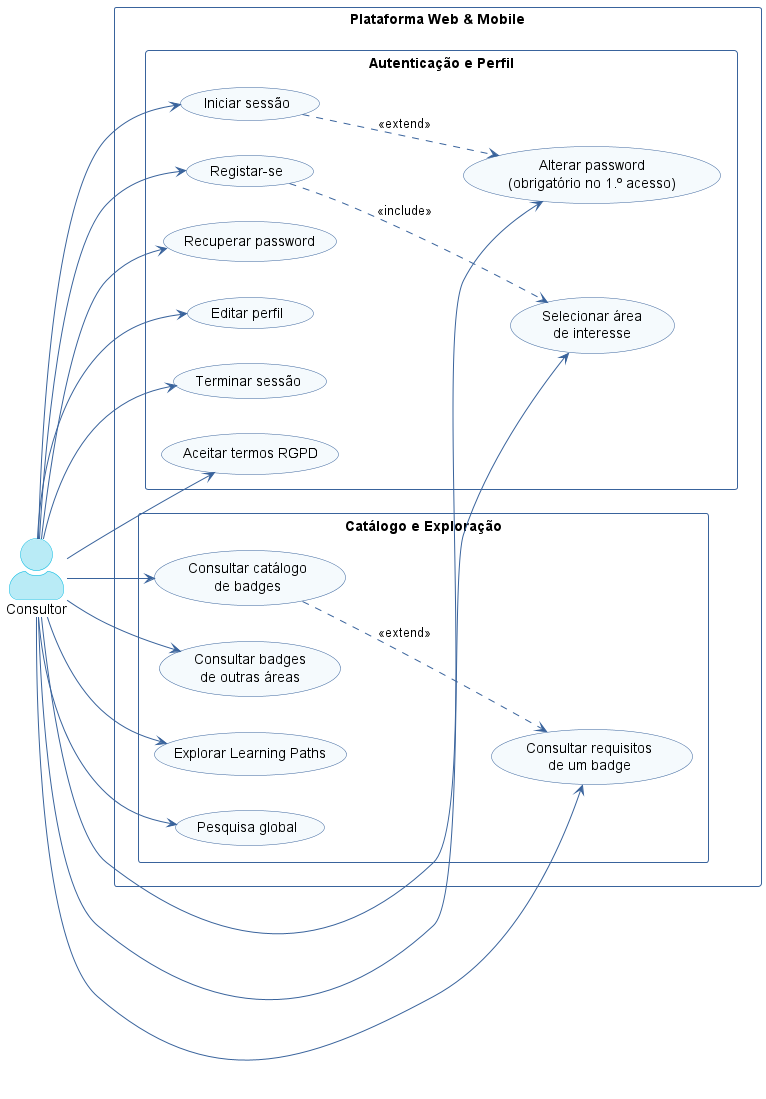
\includegraphics[width=\textwidth]{images/use-case-consultor-1.png}
  \caption{Casos de uso do Consultor --- Autenticação e Catálogo.}
  \label{fig:uc-consultor-1}
\end{figure}

\begin{figure}[H]
  \centering
  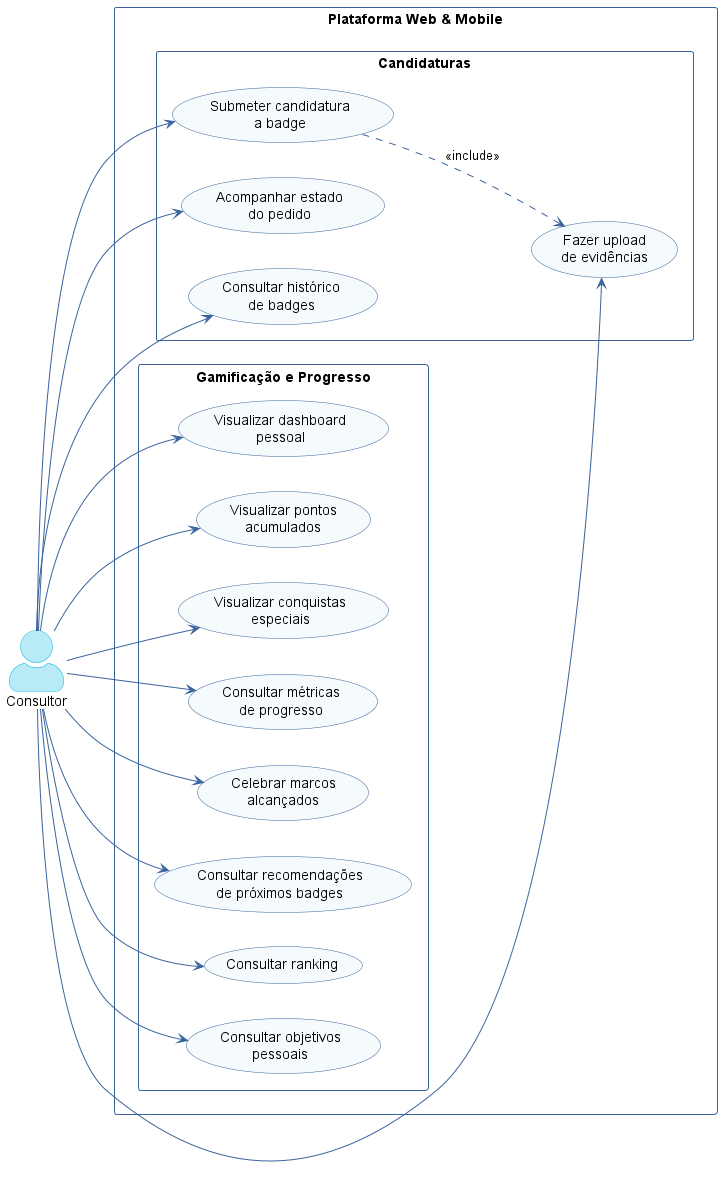
\includegraphics[width=\textwidth]{images/use-case-consultor-2.png}
  \caption{Casos de uso do Consultor --- Candidaturas e Gamificação.}
  \label{fig:uc-consultor-2}
\end{figure}

\begin{figure}[H]
  \centering
  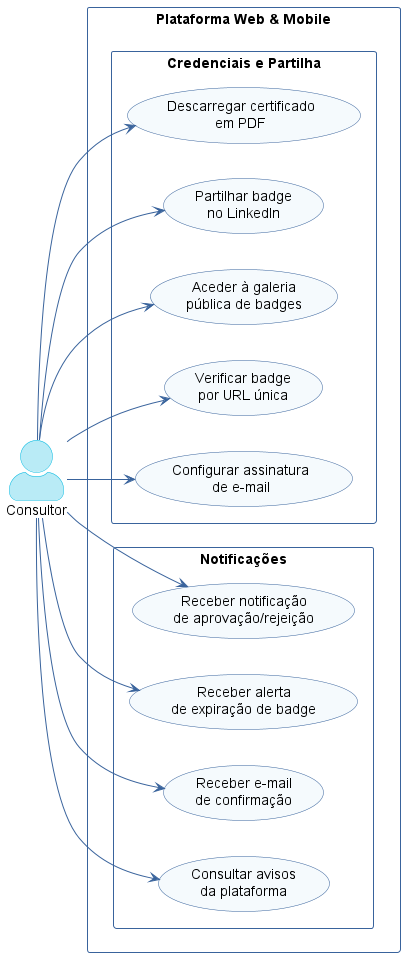
\includegraphics[width=\textwidth,height=0.5\textheight,keepaspectratio]{images/use-case-consultor-3.png}
  \caption{Casos de uso do Consultor --- Credenciais e Notificações.}
  \label{fig:uc-consultor-3}
\end{figure}

\subsubsection{Service Line Leader}

O SLL atua como validador final das candidaturas, com atuação restrita à sua Service Line. A Figura~\ref{fig:uc-sll-1} apresenta as operações de autenticação e consulta do catálogo. A Figura~\ref{fig:uc-sll-2} detalha o fluxo de validação de candidaturas e o acesso ao dashboard da sua área. A Figura~\ref{fig:uc-sll-3} cobre as funcionalidades de exportação de relatórios e notificações.

\begin{figure}[H]
  \centering
  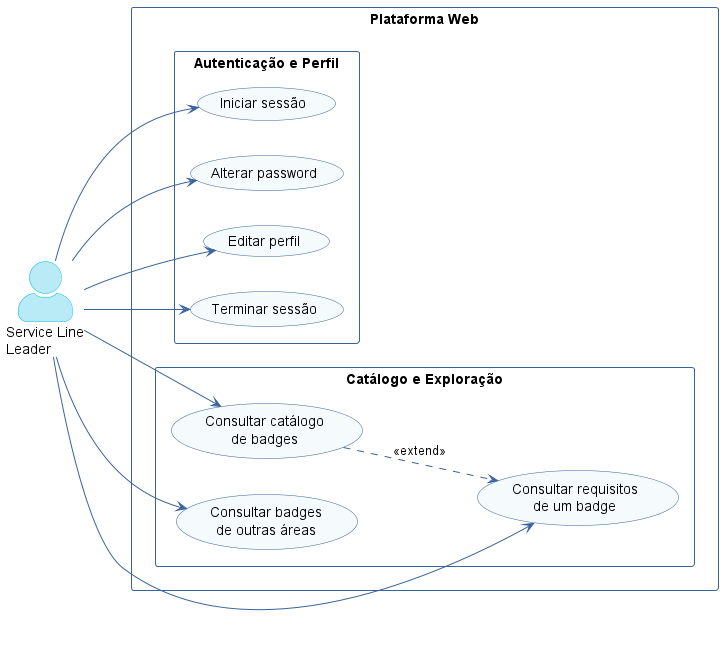
\includegraphics[width=\textwidth]{images/use-case-sll-1.png}
  \caption{Casos de uso do Service Line Leader --- Autenticação e Catálogo.}
  \label{fig:uc-sll-1}
\end{figure}

\begin{figure}[H]
  \centering
  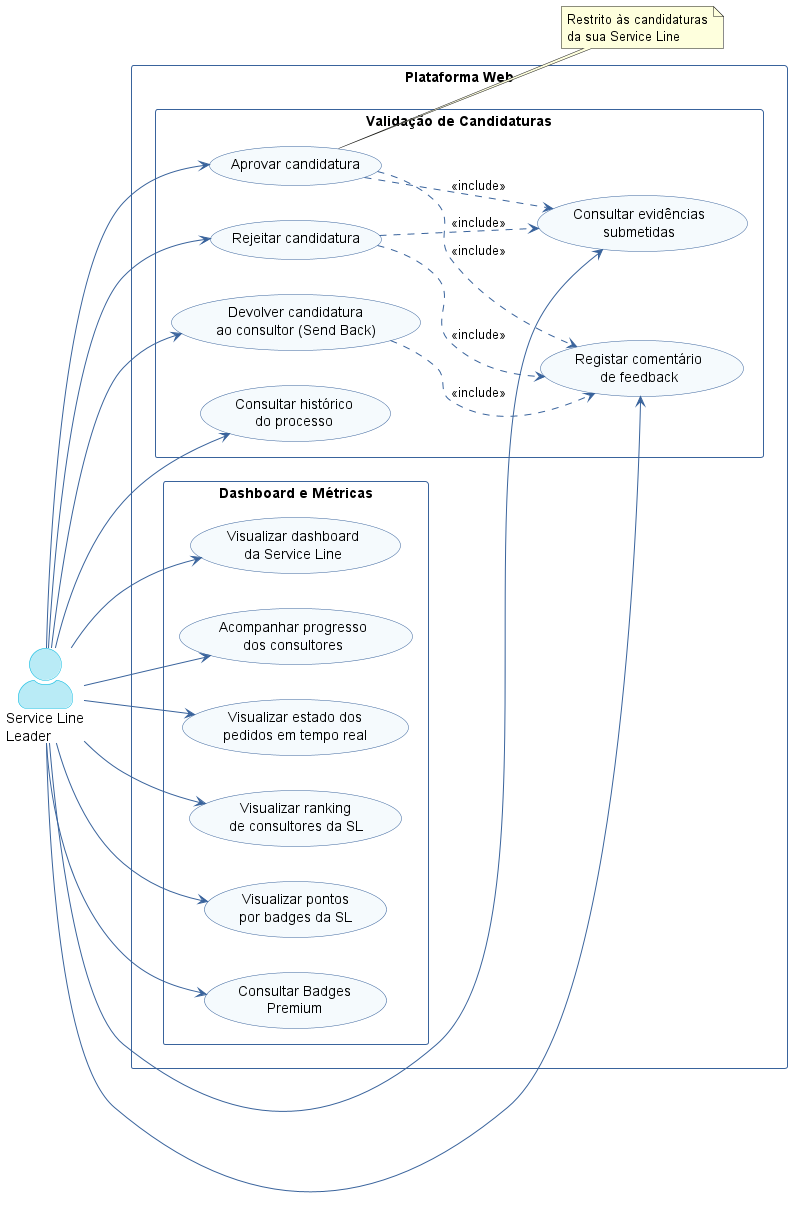
\includegraphics[width=\textwidth]{images/use-case-sll-2.png}
  \caption{Casos de uso do Service Line Leader --- Validação e Dashboard.}
  \label{fig:uc-sll-2}
\end{figure}

\begin{figure}[H]
  \centering
  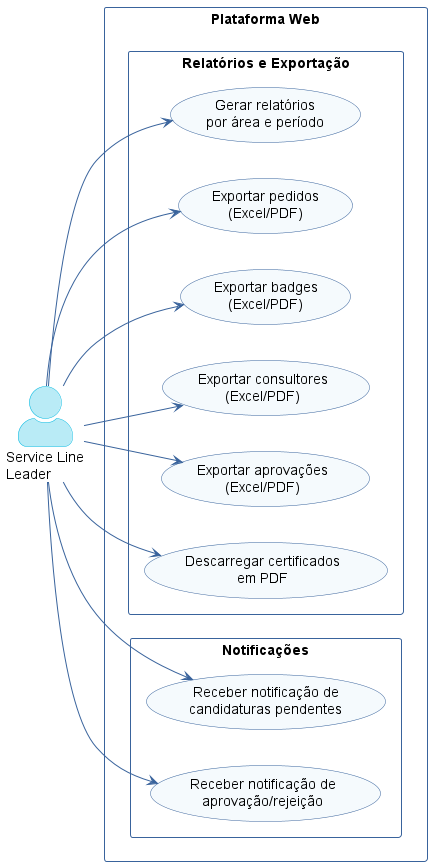
\includegraphics[width=\textwidth,height=0.5\textheight,keepaspectratio]{images/use-case-sll-3.png}
  \caption{Casos de uso do Service Line Leader --- Relatórios e Notificações.}
  \label{fig:uc-sll-3}
\end{figure}

\subsubsection{Talent Manager}

O TM desempenha o papel de primeiro validador, com atuação transversal a todas as Service Lines. A Figura~\ref{fig:uc-tm-1} ilustra as operações de autenticação e exploração do catálogo. A Figura~\ref{fig:uc-tm-2} detalha o fluxo de triagem e validação de evidências, bem como o dashboard global. A Figura~\ref{fig:uc-tm-3} apresenta as funcionalidades de exportação e notificações.

\begin{figure}[H]
  \centering
  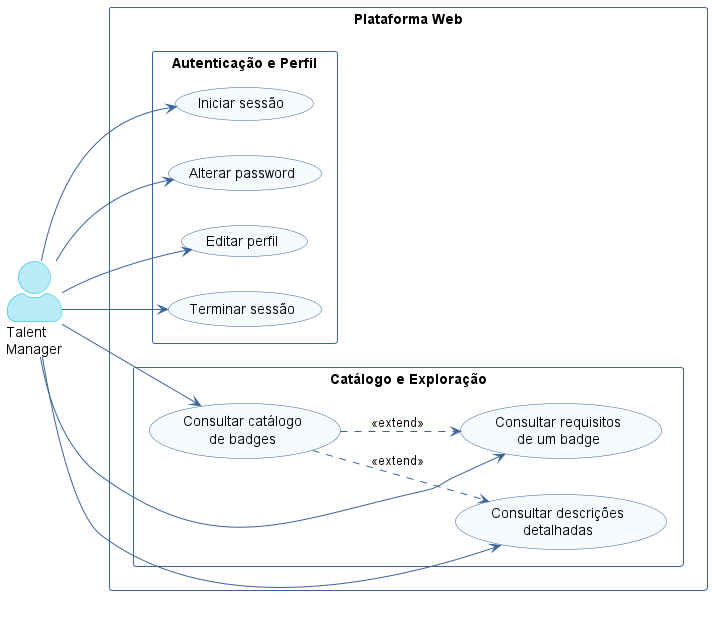
\includegraphics[width=\textwidth]{images/use-case-tm-1.png}
  \caption{Casos de uso do Talent Manager --- Autenticação e Catálogo.}
  \label{fig:uc-tm-1}
\end{figure}

\begin{figure}[H]
  \centering
  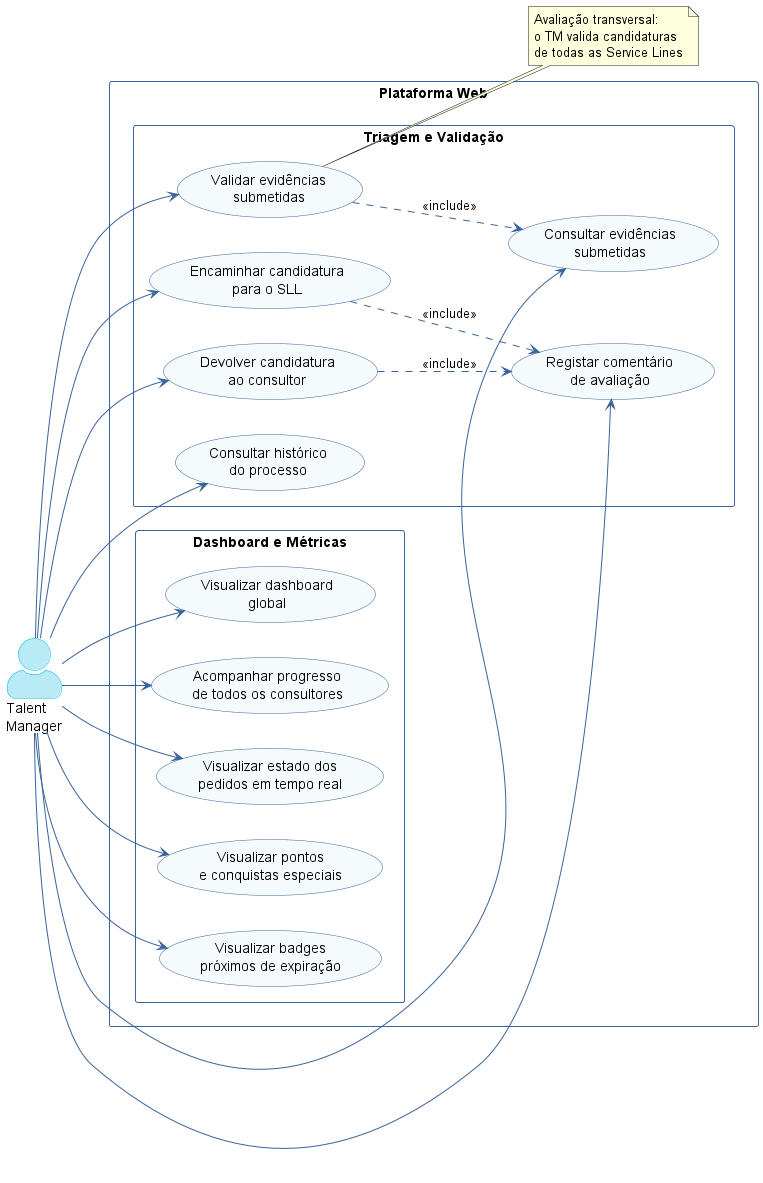
\includegraphics[width=\textwidth]{images/use-case-tm-2.png}
  \caption{Casos de uso do Talent Manager --- Triagem e Dashboard.}
  \label{fig:uc-tm-2}
\end{figure}

\begin{figure}[H]
  \centering
  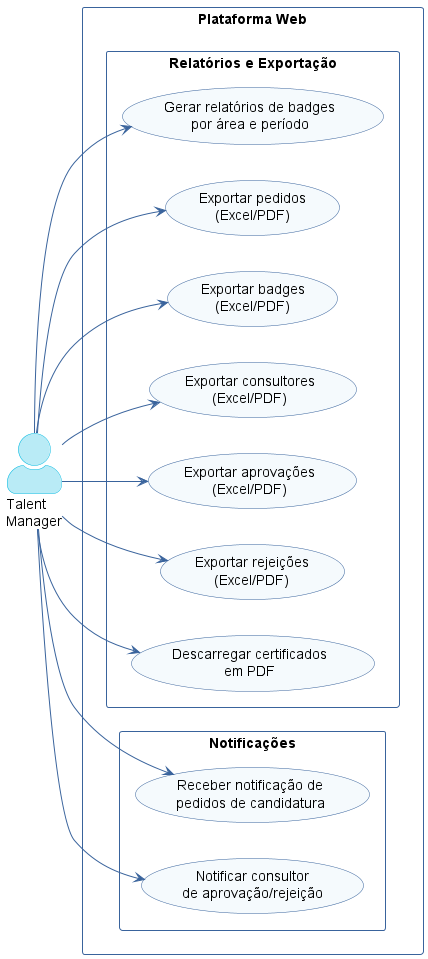
\includegraphics[width=\textwidth,height=0.5\textheight,keepaspectratio]{images/use-case-tm-3.png}
  \caption{Casos de uso do Talent Manager --- Relatórios e Notificações.}
  \label{fig:uc-tm-3}
\end{figure}

\subsubsection{Administrador}

O Administrador dispõe de acesso total à plataforma, sendo responsável pela gestão de utilizadores, conteúdos e parametrização global. A Figura~\ref{fig:uc-admin-1} abrange a autenticação, a gestão de utilizadores e a gestão da hierarquia de conteúdos. A Figura~\ref{fig:uc-admin-2} detalha a gestão de badges e o módulo de comunicação e avisos. A Figura~\ref{fig:uc-admin-3} apresenta as funcionalidades de conformidade, SLAs e exportação de dados.

\begin{figure}[H]
  \centering
  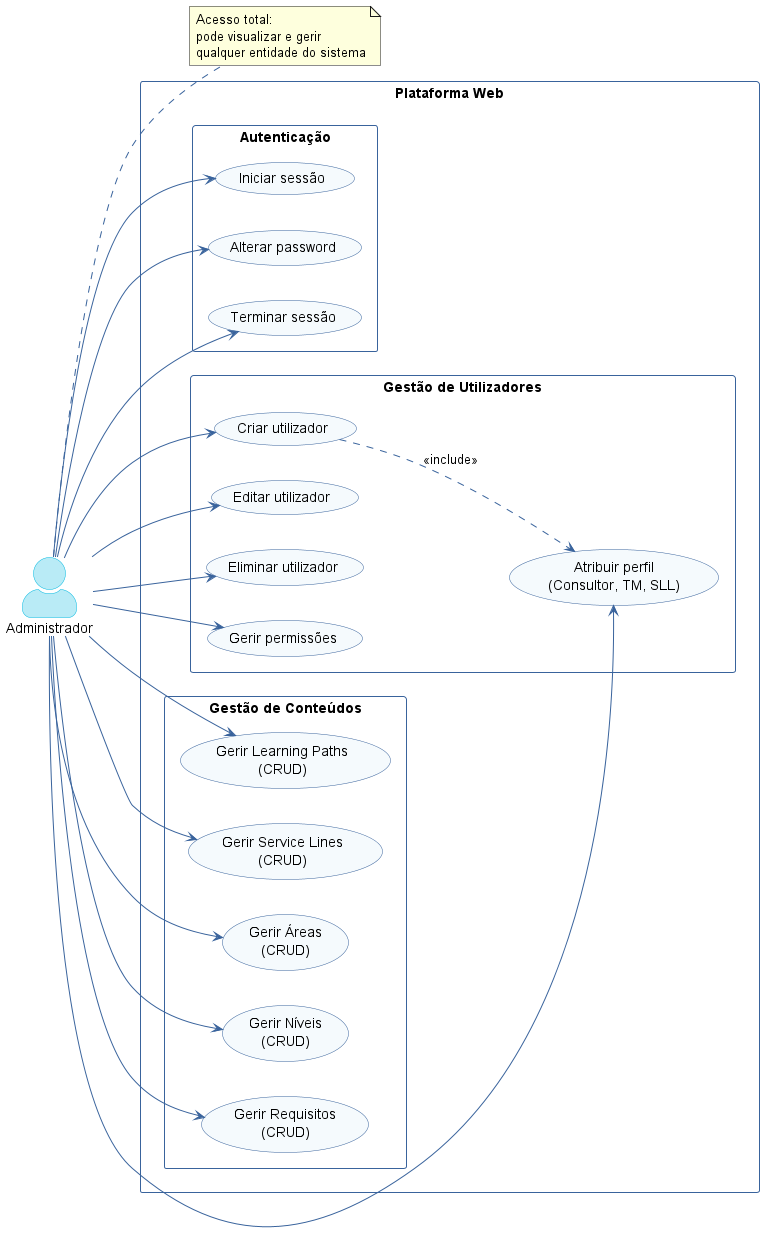
\includegraphics[width=\textwidth]{images/use-case-admin-1.png}
  \caption{Casos de uso do Administrador --- Utilizadores e Conteúdos.}
  \label{fig:uc-admin-1}
\end{figure}

\begin{figure}[H]
  \centering
  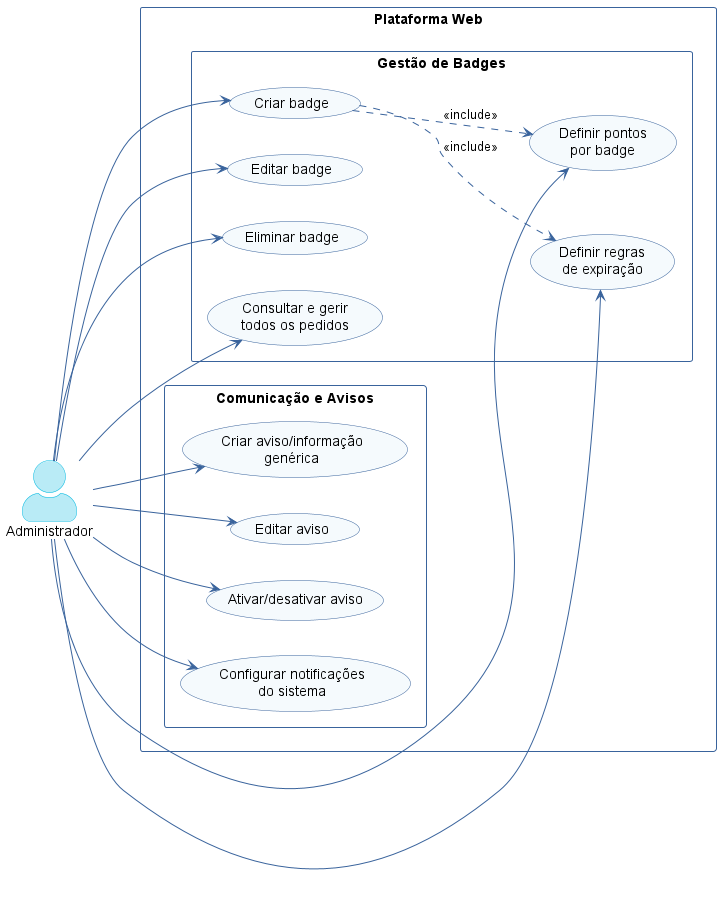
\includegraphics[width=\textwidth]{images/use-case-admin-2.png}
  \caption{Casos de uso do Administrador --- Badges e Comunicação.}
  \label{fig:uc-admin-2}
\end{figure}

\begin{figure}[H]
  \centering
  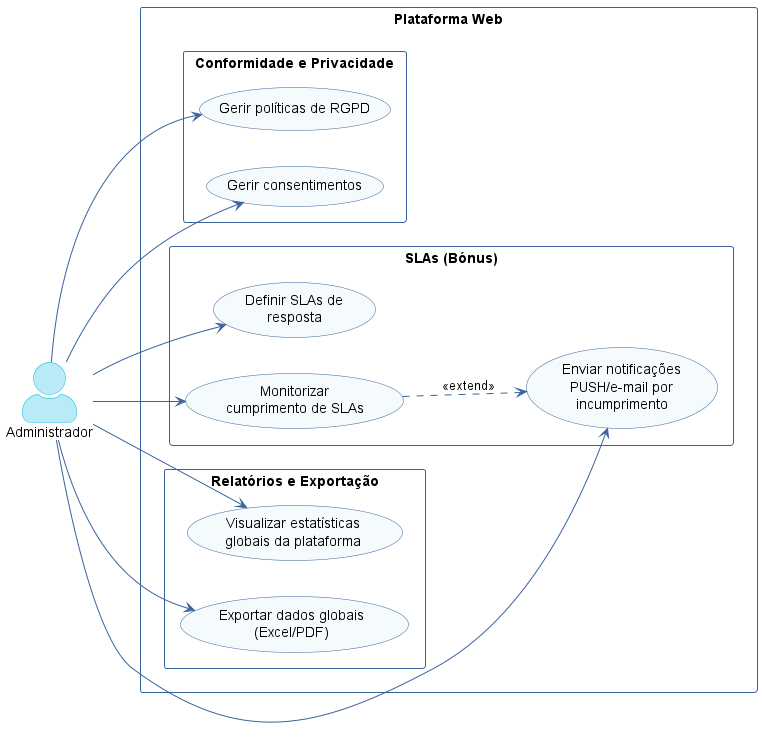
\includegraphics[width=\textwidth]{images/use-case-admin-3.png}
  \caption{Casos de uso do Administrador --- Conformidade, SLAs e Relatórios.}
  \label{fig:uc-admin-3}
\end{figure}

\section{Requisitos Não Funcionais (RNF)}

Os requisitos não funcionais definem as propriedades transversais de qualidade que o sistema deve garantir, independentemente das funcionalidades específicas de cada perfil. Foram identificadas quatro grandes áreas de preocupação: segurança, usabilidade, escalabilidade e internacionalização.

\subsection{Segurança}

A segurança foi tratada como uma prioridade estrutural desde o desenho da arquitetura até à implementação dos diferentes módulos. As medidas adotadas abrangem a comunicação, a autenticação, a autorização e a proteção dos dados pessoais.

\begin{itemize}
  \item \textbf{Encriptação de transporte:} Toda a comunicação entre o cliente e o servidor é realizada obrigatoriamente por HTTPS~\cite{restapi}, assegurada por terminação TLS ao nível do \textit{reverse proxy} de produção;
  \item \textbf{Autenticação por tokens:} O sistema utiliza JSON Web Tokens (JWT)~\cite{jwt} com o algoritmo HS256 para autenticação. O fluxo inclui \textit{access tokens} de curta duração e \textit{refresh tokens} para renovação transparente de sessões;
  \item \textbf{Alteração obrigatória de password:} No primeiro acesso após a criação da conta, o sistema força a alteração da password --- armazenada com hashing bcrypt~\cite{bcrypt} --- através de uma \textit{flag} dedicada (\texttt{fpc} --- \textit{force password change}) que bloqueia qualquer outra operação até à sua resolução;
  \item \textbf{Cabeçalhos de segurança:} A API utiliza o \textit{middleware} Helmet~\cite{helmet} para definir automaticamente cabeçalhos HTTP de proteção contra ataques comuns (XSS, \textit{clickjacking}, \textit{MIME sniffing})~\cite{owasp};
  \item \textbf{Controlo de origens (CORS):} O acesso à API é restrito a uma lista explícita de origens autorizadas, impedindo pedidos de domínios não reconhecidos;
  \item \textbf{Limitação do corpo dos pedidos:} O tamanho máximo dos corpos JSON aceites pela API está limitado a 100\,KB, prevenindo ataques de negação de serviço por \textit{payloads} volumosos. Os ficheiros de evidências são carregados diretamente para o serviço de armazenamento externo Supabase~\cite{supabase}, sem transitar pelo corpo dos pedidos;
  \item \textbf{Validação de dados de entrada:} Todos os dados recebidos pela API são validados através de esquemas Zod~\cite{zod} modulares, garantindo a conformidade dos parâmetros antes de qualquer processamento. Esta validação é replicada no lado do cliente para \textit{feedback} imediato ao utilizador;
  \item \textbf{Controlo de acesso baseado em papéis (RBAC):} Cada \textit{endpoint} da API está protegido por \textit{middleware} de verificação de papéis, assegurando que cada perfil (Administrador, Consultor, TM, SLL) apenas acede às operações que lhe são permitidas;
  \item \textbf{Conformidade com o RGPD:} O sistema dispõe de um módulo dedicado à gestão de consentimentos, exportação de dados pessoais e eliminação de contas, em conformidade com o Regulamento Geral sobre a Proteção de Dados~\cite{rgpd}.
\end{itemize}

\begin{figure}[H]
  \centering
  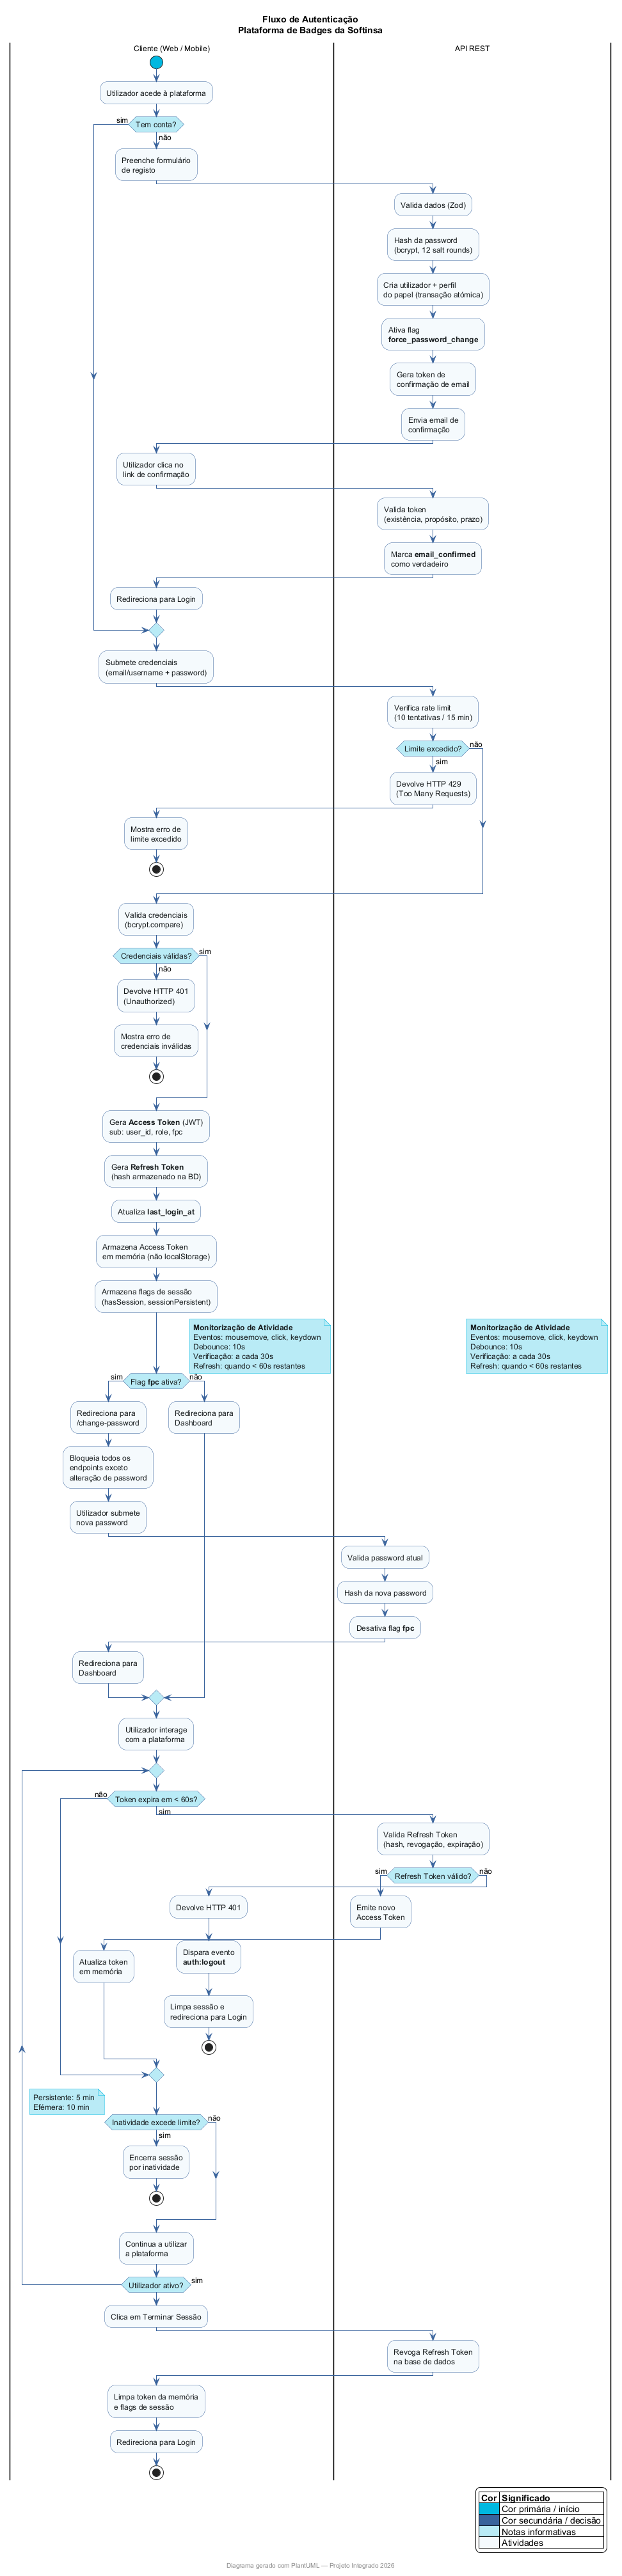
\includegraphics[width=\textwidth,height=0.85\textheight,keepaspectratio]{images/auth-flow.png}
  \caption{Fluxo completo de autenticação da plataforma.}
  \label{fig:auth-flow}
\end{figure}

\subsection{Usabilidade e Responsividade}

A interface do utilizador foi concebida para oferecer uma experiência consistente e intuitiva em qualquer dispositivo, desde ecrãs \textit{desktop} de grande dimensão até dispositivos móveis compactos.

\begin{itemize}
  \item \textbf{Design responsivo:} O portal Web utiliza o sistema de grelha do Bootstrap~\cite{bootstrap} complementado por \textit{media queries} CSS específicas, com pontos de quebra definidos para garantir a adaptação progressiva do \textit{layout} até uma largura mínima de 300\,px;
  \item \textbf{Arquitetura de componentes:} Cada componente da interface é desenvolvido num diretório próprio, contendo o ficheiro JSX e o respetivo módulo CSS (\texttt{.module.css}), promovendo a reutilização e a manutenibilidade do código;
  \item \textbf{Sistema de design:} As cores, tipografia e espaçamentos são centralizados num ficheiro de variáveis CSS globais (\texttt{colors.css}), garantindo coerência visual em toda a aplicação e facilitando alterações futuras à identidade gráfica;
  \item \textbf{Dashboards diferenciados por perfil:} Cada papel de utilizador dispõe de um dashboard dedicado, adaptado às suas necessidades específicas e apresentando apenas a informação e as ações relevantes para o seu contexto;
  \item \textbf{Validação visual de campos:} Os campos de formulário com dados inválidos ou em falta são assinalados com uma identificação a vermelho, acompanhada de mensagens de erro específicas por campo, conforme definido no enunciado;
  \item \textbf{Orientação fixa na aplicação móvel:} A aplicação Mobile está bloqueada em modo retrato, assegurando uma experiência de utilização otimizada e consistente em todos os dispositivos móveis;
  \item \textbf{Acessibilidade:} As animações da interface respeitam a preferência do sistema operativo \texttt{prefers-reduced-motion}, reduzindo ou eliminando transições para utilizadores que assim o configurem.
\end{itemize}

% TODO: Inserir capturas de ecrã comparativas (desktop vs. mobile) — ficheiros: images/responsive-*.png

\subsection{Escalabilidade}

A arquitetura do sistema foi desenhada com vista à expansão futura, tanto ao nível dos conteúdos como da base de utilizadores.

\begin{itemize}
  \item \textbf{Modelo de dados hierárquico e extensível:} A base de dados organiza os conteúdos numa estrutura hierárquica de Learning Paths, Service Lines, Áreas, Níveis e Requisitos. Esta modelação permite a introdução de novos itinerários de aprendizagem (como o futuro LP de \textit{Power Skills}) sem necessidade de alterações ao esquema relacional;
  \item \textbf{Encaminhamento hierárquico na API:} A API suporta rotas aninhadas que refletem diretamente a hierarquia do modelo de dados, permitindo o acesso contextualizado a qualquer nível da árvore de conteúdos;
  \item \textbf{Modularidade da base de código:} A API, construída sobre Express~\cite{expressjs} e o ORM Sequelize~\cite{sequelize}, está organizada em módulos independentes (rotas, controladores, serviços e validações), facilitando a adição de novas funcionalidades sem impacto nas existentes;
  \item \textbf{Processos de fundo:} Tarefas recorrentes como a monitorização de SLAs, a verificação de expiração de badges e o envio de lembretes de objetivos são executadas por \textit{workers} autónomos baseados em node-cron~\cite{nodecron}, evitando a sobrecarga do ciclo de pedido-resposta principal.
\end{itemize}

\subsection{Internacionalização}

O suporte multilingue foi implementado de forma transversal a todas as camadas do sistema, abrangendo tanto a interface do utilizador como as mensagens de erro e os códigos de resposta da API.

\begin{itemize}
  \item \textbf{Idiomas suportados:} A plataforma disponibiliza três idiomas --- Português, Inglês e Espanhol --- configuráveis pelo utilizador nas suas preferências de perfil;
  \item \textbf{Deteção automática:} Na plataforma Web, a biblioteca react-i18next~\cite{i18next} deteta automaticamente o idioma do navegador do utilizador, aplicando Português como idioma de \textit{fallback} predefinido;
  \item \textbf{Ficheiros de localização:} As traduções estão organizadas em ficheiros JSON por idioma e por domínio (\texttt{common.json} para textos da interface e \texttt{api\_codes.json} para mensagens de erro da API), garantindo a separação de contextos e a facilidade de manutenção;
  \item \textbf{Tradução \textit{offline} na aplicação Mobile:} A aplicação móvel utiliza o serviço ML Kit Translation~\cite{mlkit} para suportar traduções mesmo sem conectividade à Internet, alinhado com a arquitetura \textit{offline-first} adotada;
  \item \textbf{Saudações dinâmicas:} O sistema implementa uma lógica de saudação contextual que apresenta \textit{``Bem-vindo!''} no primeiro acesso, \textit{``Seja bem-vindo novamente''} após uma ausência superior a 15 dias e saudações baseadas na hora do dia (\textit{``Bom dia!''}, \textit{``Boa Tarde!''}, \textit{``Boa Noite!''}) nas restantes interações, traduzidas para o idioma selecionado.
\end{itemize}

% ============================================================
% Arquitetura de Informação e Modelo de Dados
% ============================================================
\chapter{Arquitetura de Informação e Modelo de Dados}
\label{ch:arquitetura}

\section{Estrutura Hierárquica}

\section{Modelo de Dados (Diagrama Entidade-Associação / Relacional)}

% ============================================================
% Prototipagem e Design de Interface (Figma)
% ============================================================
\chapter{Prototipagem e Design de Interface (Figma)}
\label{ch:prototipagem}

\section{Conceito de Design e UI/UX}

\section{Demonstração de Ecrãs Chave}

% ============================================================
% Workflow de Aprovação e Ciclo de Vida do Pedido
% ============================================================
\chapter{Workflow de Aprovação e Ciclo de Vida do Pedido}
\label{ch:workflow}

\section{Submissão (Consultor)}

\section{Triagem e Validação de Evidências (Talent Manager)}

\section{Homologação Final (Service Line Leader)}

% ============================================================
% Funcionalidades Transversais Implementadas
% ============================================================
\chapter{Funcionalidades Transversais Implementadas}
\label{ch:funcionalidades}

\section{Mecânicas de Gamificação}

\section{Módulo de Estatísticas e Reporting}

% ============================================================
% Extras e Funcionalidades Bónus
% ============================================================
\chapter{Extras e Funcionalidades Bónus}
\label{ch:extras}

\section{Sistema de Saudações Inteligente}

\section{Mural de Avisos e Comunicação}

\section{Alertas de SLA e Notificações}

% ============================================================
% Conclusão
% ============================================================
\chapter{Conclusão}
\label{ch:conclusao}

\section{Síntese do Trabalho}

% Sintetizar o trabalho realizado.

\section{Trabalho Futuro}

% Descrever possíveis melhorias e desenvolvimentos futuros.

% ============================================================
% Bibliografia
% ============================================================
\printbibliography[heading=bibintoc,title={Referências Bibliográficas}]

% ============================================================
% Appendices (optional)
% ============================================================
% \appendix
% \chapter{Diagramas Complementares}

\end{document}
